\documentclass[12pt,a4paper]{article}

% ============================================================
% PACKAGES
% ============================================================
\usepackage[utf8]{inputenc}
\usepackage[T1]{fontenc}
\usepackage[french]{babel}
\usepackage{geometry}
\usepackage{graphicx}
\usepackage{xcolor}
\usepackage{listings}
\usepackage{booktabs}
\usepackage{array}
\usepackage{hyperref}
\usepackage{fancyhdr}
\usepackage{titlesec}
\usepackage{enumitem}
\usepackage{mdframed}
\usepackage{tikz}
\usepackage{float}

% ============================================================
% MISE EN PAGE
% ============================================================
\geometry{
  top=2.5cm,
  bottom=2.5cm,
  left=2.5cm,
  right=2.5cm
}

% ============================================================
% COULEURS
% ============================================================
\definecolor{primary}{RGB}{30, 100, 180}
\definecolor{secondary}{RGB}{240, 245, 255}
\definecolor{codebg}{RGB}{245, 245, 245}
\definecolor{codeframe}{RGB}{200, 200, 200}
\definecolor{success}{RGB}{39, 174, 96}
\definecolor{warning}{RGB}{230, 126, 34}
\definecolor{darkgray}{RGB}{60, 60, 60}

% ============================================================
% EN-TETE ET PIED DE PAGE
% ============================================================
\pagestyle{fancy}
\fancyhf{}
\fancyhead[L]{\small\textcolor{primary}{\textbf{Projet M1 GIL -- Gestion de Flotte}}}
\fancyhead[R]{\small\textcolor{darkgray}{Universite de Rouen | 2025--2026}}
\fancyfoot[C]{\thepage}
\renewcommand{\headrulewidth}{0.4pt}

% ============================================================
% STYLE DES TITRES
% ============================================================
\titleformat{\section}
  {\Large\bfseries\color{primary}}
  {\thesection.}{0.8em}{}[\titlerule]

\titleformat{\subsection}
  {\large\bfseries\color{darkgray}}
  {\thesubsection.}{0.6em}{}

\titleformat{\subsubsection}
  {\normalsize\bfseries\color{darkgray}}
  {\thesubsubsection.}{0.5em}{}

% ============================================================
% STYLE DU CODE
% ============================================================
\lstset{
  backgroundcolor=\color{codebg},
  frame=single,
  rulecolor=\color{codeframe},
  basicstyle=\ttfamily\small,
  keywordstyle=\color{primary}\bfseries,
  commentstyle=\color{gray}\itshape,
  stringstyle=\color{success},
  breaklines=true,
  showstringspaces=false,
  numbers=left,
  numberstyle=\tiny\color{gray},
  numbersep=8pt,
  tabsize=2,
  captionpos=b
}

% ============================================================
% BOITE INFO
% ============================================================
\newmdenv[
  backgroundcolor=secondary,
  linecolor=primary,
  linewidth=1.5pt,
  leftline=true,
  rightline=false,
  topline=false,
  bottomline=false,
  innerleftmargin=10pt,
  innerrightmargin=10pt,
  innertopmargin=8pt,
  innerbottommargin=8pt
]{infobox}

% ============================================================
% COMMANDE PLACEHOLDER SCREENSHOT
% ============================================================
\newcommand{\screenshot}[2]{%
  \begin{figure}[H]
    \centering
    \begin{tikzpicture}
      \draw[dashed, color=gray, line width=1pt]
        (0,0) rectangle (14cm, 5cm);
      \node[color=gray] at (7cm, 2.7cm)
        {\large\textbf{[ CAPTURE D'ECRAN ]}};
      \node[color=gray] at (7cm, 2.1cm)
        {\normalsize #1};
    \end{tikzpicture}
    \caption{#2}
  \end{figure}
}

% ============================================================
% DOCUMENT
% ============================================================
\begin{document}

% ------------------------------------------------------------
% PAGE DE TITRE
% ------------------------------------------------------------
\begin{titlepage}
  \centering
  \vspace*{1cm}

  {\Large\textbf{Universite de Rouen Normandie}\\[0.3cm]
  \large Master 1 -- Genie Informatique et Logiciel}

  \vspace{1.5cm}
  \rule{\linewidth}{0.5mm}\\[0.4cm]

  {\Huge\bfseries\color{primary} Projet Gestion de Flotte de véhicules\\[0.3cm]}
  {\LARGE\bfseries Rapport de Semaine 2}\\[0.3cm]
  {\large\color{darkgray} Infrastructure DevOps -- Conteneurisation \& Orchestration}

  \rule{\linewidth}{0.5mm}\\[1.5cm]

  \begin{minipage}{0.45\textwidth}
    \begin{flushleft}
      \textbf{Etudiant :}\\
      Ahcene Amouchas \\
      Florian Pepin \\[0.5cm]
      \textbf{Encadrants :}\\
      Lydia \& Luc
    \end{flushleft}
  \end{minipage}
  \hfill
  \begin{minipage}{0.45\textwidth}
    \begin{flushright}
      \textbf{Annee universitaire :}\\
      2025 -- 2026\\[0.5cm]
      \textbf{Semaine :}\\
      2 / 7
    \end{flushright}
  \end{minipage}

  \vfill
  {\large\today}
\end{titlepage}

% ------------------------------------------------------------
% TABLE DES MATIERES
% ------------------------------------------------------------
\tableofcontents
\newpage

% ------------------------------------------------------------
% INTRODUCTION
% ------------------------------------------------------------
\section{Introduction et objectifs de la semaine}

\begin{infobox}
\textbf{Objectif de la semaine 2 :} Mettre en place l'integralite de l'environnement
d'infrastructure avant d'ecrire la moindre ligne de code metier. Cette semaine constitue
le socle sur lequel tous les microservices seront deployes dans les semaines suivantes.
\end{infobox}

\vspace{0.5cm}

La semaine 2 du projet est consacree a la mise en place de l'infrastructure DevOps
complete. L'objectif est de disposer, en fin de semaine, d'un environnement reproductible
et fonctionnel sur lequel n'importe quel membre de l'equipe peut travailler sans
configuration manuelle.

Les grandes etapes realisees sont les suivantes :

\begin{enumerate}[leftmargin=*, label=\textbf{\arabic*.}]
  \item Conteneurisation des services avec \textbf{Docker} (Dockerfiles multi-stage)
  \item Orchestration locale avec \textbf{Kubernetes} via Minikube
  \item Mise en place des manifests Kubernetes (Deployments, Services, Secrets, Ingress)
  \item Deploiement de l'infrastructure lourde via \textbf{Helm} (PostgreSQL, Redis)
  \item Resolution du probleme de deploiement de \textbf{Kafka}
  
\end{enumerate}

% ------------------------------------------------------------
% SECTION - ENVIRONNEMENT DE DEVELOPPEMENT LOCAL
% ------------------------------------------------------------
\section{Environnement de developpement local -- Docker Compose}

\begin{infobox}
\textbf{Principe :} Docker Compose sert uniquement au developpement rapide en local.
Kubernetes (Minikube) simule l'environnement de production. Les deux sont independants
et ne se parlent pas.
\end{infobox}

\vspace{0.3cm}

A la racine du projet, un fichier \texttt{docker-compose.yml} permet de lancer
instantanement toute l'infrastructure necessaire au developpement sans passer par
Kubernetes. Il contient 5 services :

\begin{table}[H]
  \centering
  \begin{tabular}{llll}
    \toprule
    \textbf{Conteneur} & \textbf{Image} & \textbf{Port} & \textbf{Role} \\
    \midrule
    flotte-postgres  & timescale/timescaledb:2.14.2-pg15    & 5432 & Base de donnees principale + time-series \\
    flotte-redis     & redis:7.2-alpine                     & 6379 & Cache et service evenements \\
    flotte-kafka     & apache/kafka:3.7.0                   & 9092 & Bus de messages (mode KRaft) \\
    flotte-keycloak  & keycloak:24.0.2  & 8180 & Authentification SSO \\
    flotte-pgadmin   & dpage/pgadmin4                       & 5050 & Interface web PostgreSQL \\
    \bottomrule
  \end{tabular}
  \caption{Services du Docker Compose de developpement local}
\end{table}

\textbf{Choix techniques notables :}
\begin{itemize}
  \item \textbf{TimescaleDB} a la place de PostgreSQL standard -- supporte nativement
        les donnees time-series pour le service de localisation GPS
  \item \textbf{Kafka en mode KRaft} -- sans Zookeeper, architecture simplifiee
  \item \textbf{Keycloak} integre des le developpement local pour tester
        l'authentification SSO sans attendre Kubernetes
\end{itemize}

\begin{infobox}
\textbf{Note :} Deux images Kafka differentes sont utilisees selon l'environnement :
\texttt{apache/kafka:3.7.0} en developpement local (Docker Compose) et
\texttt{confluentinc/cp-kafka:7.5.0} sur Kubernetes. Ce choix est volontaire --
l'image Apache etant disponible sur Docker Hub pour le dev local, et l'image
Confluent etant plus stable pour l'orchestration Kubernetes. Le protocole Kafka
etant standardise, les deux sont entierement compatibles.
\end{infobox}

Le lancement se fait en une seule commande :

\begin{lstlisting}[language=bash, caption=Lancement de l'environnement de developpement local]
docker-compose up -d
\end{lstlisting}

\begin{figure}[H]
    \centering
    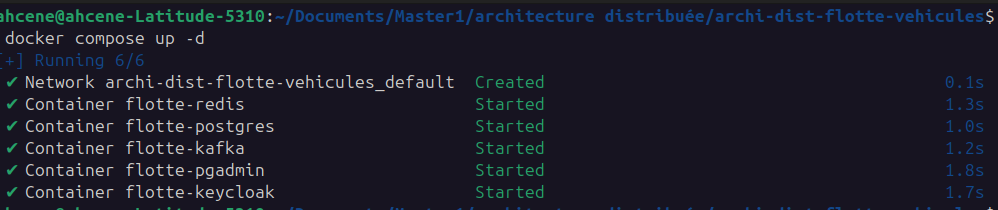
\includegraphics[width=0.8\textwidth]{docker-compose.png}
    \caption{Les 5 conteneurs du Docker Compose demarres et operationnels}
    \label{fig:docker-compose}
\end{figure}

pgAdmin est accessible sur \texttt{http://localhost:5050} et Keycloak sur
\texttt{http://localhost:8080}. Ces interfaces permettent de visualiser et administrer
les donnees sans ligne de commande pendant le developpement.

% ------------------------------------------------------------
% SECTION 1 - DOCKER
% ------------------------------------------------------------
\section{Conteneurisation avec Docker}

\subsection{Concept}

Docker permet d'empaqueter une application et toutes ses dependances dans une image
standardisee, garantissant qu'elle fonctionnera de maniere identique sur n'importe quel
environnement (poste de developpement, CI/CD, production).

\subsection{Dockerfile multi-stage pour vehicle-service}

Le choix d'un \textbf{Dockerfile multi-stage} permet de separer la phase de compilation
de la phase d'execution, reduisant ainsi la taille de l'image finale et ameliorant la
securite en n'incluant pas les outils de build en production.


\begin{lstlisting}[language=bash, caption=Dockerfile multi-stage – vehicle-service (Spring Boot)]
# Etape 1 : Construction
FROM maven:3.9.6-eclipse-temurin-21-alpine AS builder

WORKDIR /build

# On copie d'abord le pom.xml pour telecharger les dependances
COPY pom.xml .
RUN mvn dependency:go-offline

# On copie tout le code source et on compile le projet
COPY src ./src
RUN mvn clean package -DskipTests

# Etape 2 : Production
FROM eclipse-temurin:21-jre-alpine

WORKDIR /app

# Securite : creation d'un utilisateur non-root
RUN addgroup -S spring && adduser -S spring -G spring
USER spring:spring

# On recupere l'application compilee depuis l'etape 1
COPY --from=builder /build/target/*.jar app.jar

# On expose le port de Spring Boot
EXPOSE 8080

# Commande de lancement
ENTRYPOINT ["java", "-jar", "app.jar"]
\end{lstlisting}

\textbf{Points cles du Dockerfile :}
\begin{itemize}
  \item \texttt{imagePullPolicy: Never} -- obligatoire en local pour utiliser les images
        construites directement dans l'environnement Docker de Minikube
  \item Utilisation d'un utilisateur non-root pour la securite
  \item Separation build / production pour reduire la taille de l'image finale
\end{itemize}

\subsection{Construction de l'image dans Minikube}

Pour eviter d'avoir a pousser les images sur un registre distant (Docker Hub), les images
ont ete construites directement dans l'environnement Docker interne de Minikube :

\begin{lstlisting}[language=bash, caption=Construction de l'image dans Minikube]
# Pointer le daemon Docker vers Minikube
eval $(minikube docker-env)

# Builder l'image directement dans Minikube
docker build -t vehicle-service:latest ./services/vehicle-service/

# Verifier que l'image est disponible
minikube image ls | grep vehicle
\end{lstlisting}


\begin{figure}[h]
    \centering
    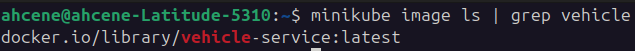
\includegraphics[width=0.8\textwidth]{minikube.png}
    \caption{Construction de l'image vehicle-service dans Minikube}
    \label{fig:login}
\end{figure}
% ------------------------------------------------------------
% SECTION 2 - KUBERNETES
% ------------------------------------------------------------
\section{Orchestration avec Kubernetes (Minikube)}

\subsection{Concept}

Kubernetes est le chef d'orchestre des conteneurs. Il garantit que les services restent
disponibles (redemarrage automatique en cas de crash), gere le reseau interne entre
services, et permet la mise a l'echelle. \textbf{Minikube} simule un cluster Kubernetes
professionnel sur une seule machine locale.

\subsection{Isolation du projet -- Namespace}

Un \textbf{Namespace} a ete cree pour isoler l'integralite du projet dans un espace
dedie, separe du reste du systeme Kubernetes :

\begin{lstlisting}[language=bash, caption=Creation du namespace]
kubectl apply -f infra/kubernetes/namespaces/namespace.yaml
kubectl get namespaces
\end{lstlisting}

\subsection{Les 4 objets Kubernetes mis en place}

\subsubsection{Deployment -- Gestion des conteneurs}

Le \textbf{Deployment} declare quoi faire tourner, combien de replicas maintenir, et
relance automatiquement les pods en cas de crash. Un Deployment a ete cree pour chacun
des 5 microservices avec 2 replicas chacun.

\begin{figure}[h]
    \centering
    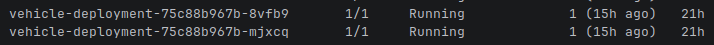
\includegraphics[width=0.8\textwidth]{vehicle-pod.png}
    \caption{Exemple de Deployment Kubernetes -- vehicle-service}
    \label{fig:login}
\end{figure}

\subsubsection{Service -- Adresse reseau stable}

Les pods etant ephemeres (leur IP change a chaque redemarrage), le \textbf{Service}
Kubernetes fournit une adresse reseau stable et permanente. Tous les services sont de
type \texttt{ClusterIP} (accessibles uniquement en interne au cluster).

\begin{table}[H]
  \centering
  \begin{tabular}{llcc}
    \toprule
    \textbf{Service} & \textbf{Technologie} & \textbf{Port} & \textbf{Type} \\
    \midrule
    vehicle-service     & Spring Boot & 8080 & ClusterIP \\
    driver-service      & Spring Boot & 8081 & ClusterIP \\
    maintenance-service & Spring Boot & 8082 & ClusterIP \\
    event-service       & Spring Boot & 8083 & ClusterIP \\
    location-service    & Node.js     & 3000 & ClusterIP \\
    \bottomrule
  \end{tabular}
  \caption{Recapitulatif des Services Kubernetes deployes}
\end{table}

\subsubsection{Secret -- Gestion securisee des mots de passe}

Les mots de passe et URLs de connexion ne sont jamais ecrits en dur dans le code source
ni dans les Deployments. Un \textbf{Secret Kubernetes} centralise ces donnees sensibles
et les injecte comme variables d'environnement dans les pods au demarrage.

Dans le fichier \texttt{application.yaml} de Spring Boot, la syntaxe
\texttt{\$\{VARIABLE:valeur\_defaut\}} permet d'utiliser la variable injectee par le
Secret, avec une valeur de fallback pour le developpement local :

\begin{lstlisting}[language=bash, caption=application.yaml -- injection des secrets via variables d'environnement]
spring:
  datasource:
    url: ${SPRING_DATASOURCE_URL:jdbc:postgresql://localhost:5432/flotte_db}
    username: ${SPRING_DATASOURCE_USERNAME:admin}
    password: ${SPRING_DATASOURCE_PASSWORD:password}
  kafka:
    bootstrap-servers: ${KAFKA_BROKER:localhost:9092}
\end{lstlisting}

Le fichier \texttt{db-secrets.yaml} est ajoute au \texttt{.gitignore} pour ne jamais
etre commite sur Git. Un fichier \texttt{values.secret.yaml.example} sert de template
pour les membres de l'equipe.

\subsubsection{Ingress -- Point d'entree externe}

L'\textbf{Ingress} expose le cluster vers l'exterieur et route les requetes HTTP vers
le bon service selon le chemin URL. Le controller NGINX a ete active via l'addon Minikube :

\begin{lstlisting}[language=bash, caption=Activation et configuration de l'Ingress]
# Activer l'addon Ingress NGINX
minikube addons enable ingress

# Ajouter fleet.local dans /etc/hosts
echo "$(minikube ip) flotte.local" | sudo tee -a /etc/hosts

# Appliquer le manifest
kubectl apply -f infra/kubernetes/ingress/ingress.yaml
\end{lstlisting}

\begin{figure}[h]
    \centering
    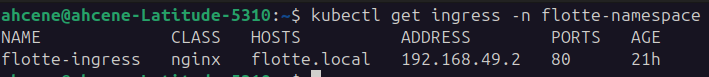
\includegraphics[width=0.8\textwidth]{ingress.png}
    \caption{Ingress deploye avec l'adresse IP de Minikube}
    \label{fig:login}
\end{figure}

La table de routage configuree est la suivante :

\begin{table}[H]
  \centering
  \begin{tabular}{ll}
    \toprule
    \textbf{URL} & \textbf{Service cible} \\
    \midrule
    \texttt{fleet.local/api/vehicles}    & vehicle-service:8080 \\
    \texttt{fleet.local/api/drivers}     & driver-service:8081 \\
    \texttt{fleet.local/api/maintenance} & maintenance-service:8082 \\
    \texttt{fleet.local/api/events}      & event-service:8083 \\
    \texttt{fleet.local/api/location}    & location-service:3000 \\
    \bottomrule
  \end{tabular}
  \caption{Table de routage de l'Ingress}
\end{table}

% ------------------------------------------------------------
% SECTION 3 - HELM
% ------------------------------------------------------------
\section{Infrastructure as Code avec Helm}

\subsection{Concept}

Helm est le gestionnaire de paquets de Kubernetes. Plutot que d'ecrire et maintenir
manuellement des dizaines de fichiers YAML pour des services tiers complexes, Helm utilise
des \textbf{Charts} -- des packages preconfigures et maintenus par la communaute.

\subsection{Strategie de deploiement}

Une separation stricte a ete mise en place entre :

\begin{itemize}
  \item \textbf{Infrastructure lourde} (PostgreSQL, Redis) : deployee via Helm Charts Bitnami
  \item \textbf{Microservices applicatifs} : deployes via des manifests Kubernetes classiques
\end{itemize}

Cela permet a n'importe quel developpeur de lancer toute l'infrastructure en
\textbf{3 commandes seulement} :

\begin{lstlisting}[language=bash, caption=Lancement complet de l'infrastructure]
helm dependency update ./infra/helm/dependencies/
helm upgrade --install infra-stack ./infra/helm/dependencies/ \
  --namespace flotte-namespace \
  -f values.yaml \
  -f values.secret.yaml
kubectl apply -f infra/kubernetes/ -R
\end{lstlisting}

\subsection{Separation des secrets Helm}

Pour ne pas exposer les mots de passe sur Git, une approche a deux fichiers a ete adoptee :

\begin{itemize}
  \item \texttt{values.yaml} -- configuration non-sensible, commite sur Git
  \item \texttt{values.secret.yaml} -- mots de passe uniquement, dans \texttt{.gitignore}
  \item \texttt{values.secret.yaml.example} -- template pour les coeequipiers, commite sur Git
\end{itemize}

\begin{figure}[h]
    \centering
    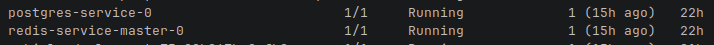
\includegraphics[width=0.8\textwidth]{pod-bdd.png}
    \caption{PostgreSQL et Redis deployes et Running via Helm Bitnami}
    \label{fig:login}
\end{figure}

% ------------------------------------------------------------
% SECTION 4 - KAFKA
% ------------------------------------------------------------
\section{Resolution du probleme Kafka }

\subsection{Probleme rencontre}

Le deploiement de Kafka via le Chart Helm Bitnami a echoue avec l'erreur
\texttt{Init:ImagePullBackOff}. L'investigation via \texttt{kubectl describe pod} a
revele la cause exacte :

\begin{lstlisting}[language=bash, caption=Message d'erreur lors du describe pod]
Warning Failed  kubelet  Failed to pull image "bitnami/kafka:3.7.0":
Error response from daemon: manifest unknown: manifest unknown
\end{lstlisting}

\textbf{Cause identifiee :} Bitnami a retire ses images de Docker Hub depuis 2023.
Les tags versionnels (\texttt{bitnami/kafka:3.7.0}, \texttt{latest}) n'existent plus
sur les registres publics accessibles depuis Minikube.


\subsection{Pivot technique -- Image Confluent officielle}

Plutot que de s'acharner sur un outil instable, la decision a ete prise d'abandonner
le Chart Bitnami pour Kafka et d'utiliser un manifest Kubernetes classique avec l'image
officielle \textbf{Confluent Platform} (\texttt{confluentinc/cp-kafka:7.5.0}),
equivalent a Apache Kafka 3.5.x.

\textbf{Avantages de cette approche :}
\begin{itemize}
  \item Configuration en mode \textbf{KRaft} (sans Zookeeper) -- architecture simplifiee
  \item Image Confluent, reference industrielle utilisee en production
  \item Controle total de la configuration via variables d'environnement
  \item Demarrage instantane, pas d'init containers problematiques
\end{itemize}

\begin{lstlisting}[language=bash, caption=Solution -- deploiement Kafka via manifest Kubernetes]
# Deploiement via manifest classique avec image Confluent
kubectl apply -f infra/kubernetes/kafka/kafka.yaml

# Verification que Kafka tourne
kubectl get pods -n flotte-namespace | grep kafka
\end{lstlisting}

\begin{figure}[h]
    \centering
    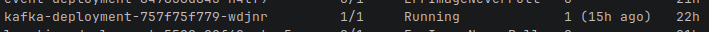
\includegraphics[width=0.8\textwidth]{pod-kafka.png}
    \caption{Kafka deploye et Running via manifest Kubernetes -- image confluentinc/cp-kafka:7.5.0 (Kafka 3.5)}
    \label{fig:login}
\end{figure}
% ------------------------------------------------------------
% SECTION 5 - BILAN
% ------------------------------------------------------------
\section{Bilan de la semaine 2}

\subsection{Etat final du cluster}
\textbf{Voici l'etat du cluster pour le moment :}
\begin{figure}[h]
    \centering
    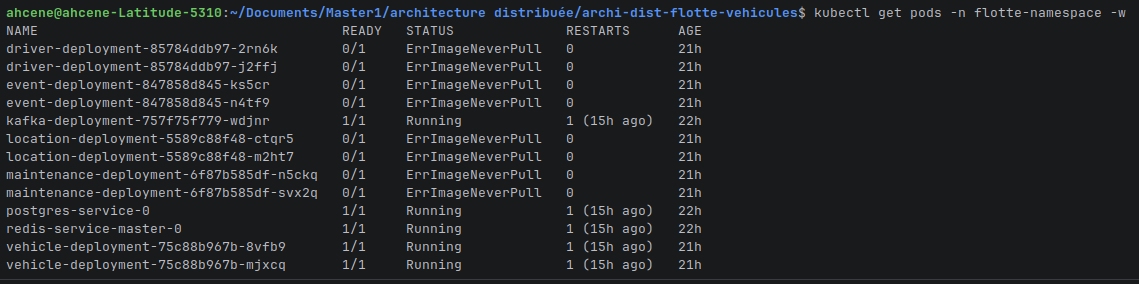
\includegraphics[width=0.8\textwidth]{pods.png}
    \caption{Etat final du cluster en fin de semaine 2}
    \label{fig:login}
\end{figure}

\begin{table}[H]
  \centering
  \begin{tabular}{lcc}
    \toprule
    \textbf{Composant} & \textbf{Statut} & \textbf{Methode de deploiement} \\
    \midrule
    PostgreSQL           & \textcolor{success}{\textbf{Running}} & Helm (Bitnami) \\
    Redis                & \textcolor{success}{\textbf{Running}} & Helm (Bitnami) \\
    Kafka  & \textcolor{success}{\textbf{Running}} & Manifest K8s (Confluent cp-kafka:7.5.0) \\
    vehicle-service      & \textcolor{success}{\textbf{Running}} & Manifest K8s \\
    driver-service       & \textcolor{warning}{\textbf{Pending}} & Image a builder (S3) \\
    maintenance-service  & \textcolor{warning}{\textbf{Pending}} & Image a builder (S4) \\
    location-service     & \textcolor{warning}{\textbf{Pending}} & Image a builder (S5) \\
    event-service        & \textcolor{warning}{\textbf{Pending}} & Image a builder (S4) \\
    Ingress Controller   & \textcolor{success}{\textbf{Running}} & Minikube addon NGINX \\
    \bottomrule
  \end{tabular}
  \caption{Bilan de l'etat des composants en fin de semaine 2}
\end{table}

\begin{infobox}
L'etat \texttt{ErrImageNeverPull} des services non encore developpes est
\textbf{normal et attendu} -- les images Docker n'existent pas encore car le code
metier sera ecrit lors des semaines 3 a 5. La structure Kubernetes est en place et
prete a les accueillir.
\end{infobox}

\subsection{Structure finale du projet}

\begin{lstlisting}[caption=Arborescence du projet en fin de semaine 2]
racine-du-projet/
|-- docker-compose.yml              # Env. de dev rapide (local)
|-- .env.example                    # Template variables d'environnement
|-- .gitignore                      # Inclut values.secret.yaml, db-secrets.yaml
|-- services/
|   |-- vehicle-service/            # Spring Boot (Running)
|   |   |-- Dockerfile
|   |   `-- src/
|   |-- driver-service/             # Spring Boot (a developper S3)
|   |-- maintenance-service/        # Spring Boot (a developper S4)
|   |-- location-service/           # Node.js    (a developper S5)
|   `-- event-service/              # Spring Boot (a developper S4)
`-- infra/
    |-- helm/
    |   `-- dependencies/
    |       |-- Chart.yaml          # Dependances Bitnami (Postgres, Redis)
    |       |-- values.yaml         # Config sans secrets (sur Git)
    |       |-- values.secret.yaml  # Mots de passe (hors Git)
    |       `-- values.secret.yaml.example
    `-- kubernetes/
        |-- namespaces/             # flotte-namespace
        |-- secrets/                # db-secrets.yaml (hors Git)
        |-- deployments/            # 5 microservices x 2 replicas
        |-- services/               # 5 ClusterIP services
        |-- kafka/                  # kafka.yaml (apache/kafka:3.7.0)
        `-- ingress/                # fleet.local routing
\end{lstlisting}

\subsection{Points d'attention pour la suite}

\begin{itemize}
  \item \textbf{Semaine 3 :} Coder le vehicle-service (CRUD REST, Kafka producer/consumer,
        tests unitaires $>$80\%, OpenTelemetry)
  \item \textbf{CI/CD :} Finaliser le pipeline GitHub Actions (build Docker + tests
        automatiques a chaque push)
  \item \textbf{Observabilite :} Deployer la stack OpenTelemetry, Prometheus, Grafana,
        Jaeger et Loki
  \item \textbf{Semaine 7 :} Packager les microservices dans un Chart Helm pour le
        deploiement final prod-ready
\end{itemize}

% ------------------------------------------------------------
% CONCLUSION
% ------------------------------------------------------------
\section{Conclusion}

La semaine 2 a permis de construire un environnement d'infrastructure solide et
reproductible. Le principal defi rencontre -- l'instabilite du Chart Helm Kafka de
Bitnami -- a ete resolu par un \textbf{pivot technique rapide} vers un manifest
Kubernetes classique utilisant l'image officielle Apache Kafka. Cette decision illustre
l'importance de l'agilite dans un projet d'architecture distribuee : identifier rapidement
qu'un outil pose probleme et le remplacer par une solution plus simple et plus fiable.

En fin de semaine, l'ensemble des composants d'infrastructure (PostgreSQL, Redis, Kafka,
Ingress, Secrets) est operationnel dans le cluster Minikube. Le service
\texttt{vehicle-service} tourne deja en \texttt{Running}, validant le bon fonctionnement
de la chaine complete : Dockerfile $\rightarrow$ image Minikube $\rightarrow$ Deployment
$\rightarrow$ Service $\rightarrow$ Ingress.

\vspace{1cm}
\begin{center}
\rule{0.5\linewidth}{0.4pt}\\[0.3cm]
{\small Rapport -- Projet M1 GIL -- Universite de Rouen Normandie | 2025--2026}
\end{center}

\end{document}